\chapter{SpaceRL framework}\label{chap:framework}

\chapterQuote{\textit{``Most problems can be solved using algebra, or violence.''}}{--- Bill Wurtz}

\chapterAbstract{B}{efore we delve into the details of our proposal, it is important to establish a common and unambiguous vocabulary. For this reason, we have devised a conceptual framework that allows us to describe a number of relevant concepts in detail. The chapter is organized as follows: Section \ref{sec:theo-intro} introduces it, Section \ref{sec:theo-triple} models the concept of a triple, Section \ref{sec:theo-kg} presents the theoretical model of a Knowledge Graph, Section \ref{sec:theo-paths} introduces topology-based elements such as paths, distances and reachability, Section \ref{sec:theo-subgraph} illustrates the concept of neighborhood subgraphs, Section \ref{sec:theo-candidates} presents the notions of candidate triples and candidate-filtering fitness, Section \ref{sec:theo-rule} describes candidate-filtering criteria and rules, and Section \ref{sec:theo-features} introduces graph-based features and feature groups; finally, Section \ref{sec:theo-conclusion} summarizes the chapter.}

\section{Introduction}\label{sec:theo-intro}
% Throughout our proposal, we use a number of concepts, both established in this field and novel. In this chapter, we define their foundations, such as tuples of entities and relations known as triples, or the fields of a Knowledge Graph, which allow us to accurately describe further concepts. We also define paths inside a Knowledge Graph, which are the basis for many of the elements in our proposal. Building upon the notion of a path, we provide a formal definition of the distance between two entities in a Knowledge Graph, as well as of the concept of entity reachability.

% Furthermore, in this chapter, we define neighborhood subgraphs, which are portions of a KG that contain the elements most closely related to a given entity. Then, we introduce candidate triples, which are combinations of entities and relations that have a high likelihood of representing correct knowledge. To measure the tentative aptness of a candidate triple, we present the idea of candidate fitness. In order to rule out those candidate triples with a low fitness, we define candidate filtering criteria and rules. Finally, we introduce a way to numerically model a triple in a KG through the use of graph-based feature groups.

% \begin{figure}[htp]
%     \centering
%     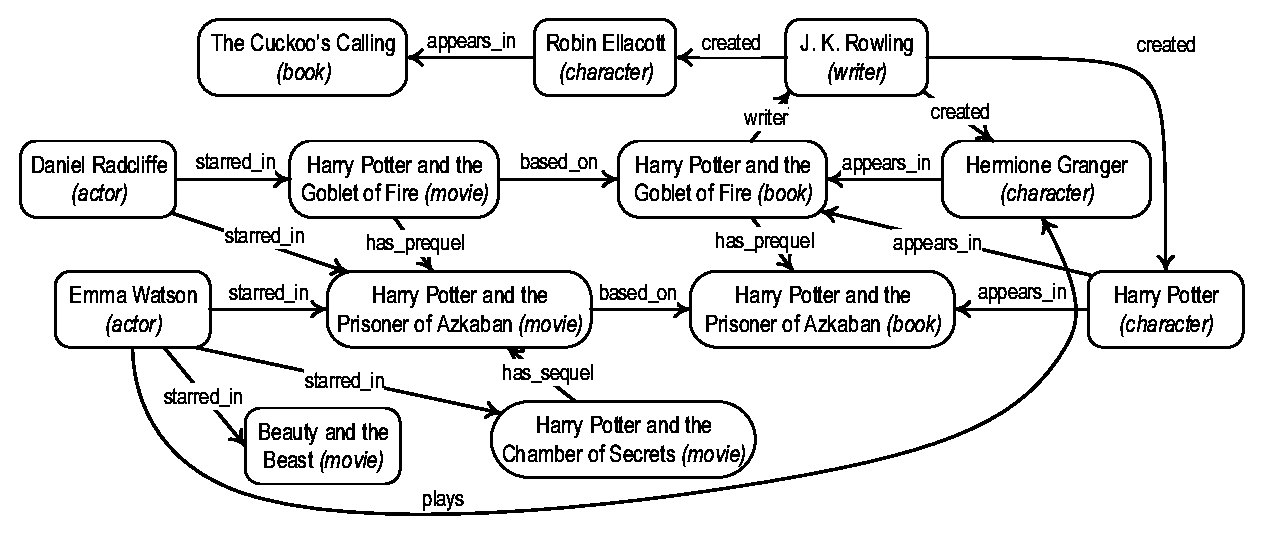
\includegraphics[width=\textwidth]{fig/theoretical/kg-harry-potter}
%     \caption{Sample KG describing works, actors, writers and characters}
%     \label{fig:kg-potter}
% \end{figure}

% To help illustrate some concepts in this chapter, Figure~\ref{fig:kg-potter} presents a KG that contains information about fictional works, actors, writers and characters.

\section{Triple}\label{sec:theo-triple}
% The notion of a triple is pivotal to Knowledge Graphs, since it constitutes an atomical amount of structured information. A triple is a 3-tuple that contains two entities, commonly denoted \textit{source} and \textit{target}\footnote{Other literature sometimes refers to the two entities in a triple as \textit{head} and \textit{tail} \cite{dessi2022cskg,dessi2020aikg,bordes2013}, or \textit{subject} and \textit{object} \cite{nickel2016, balazevic2019,trouillon2016}.}; connected by means of a relation. This, in turn, represents a fact in a given domain.

% Formally, a triple is defined as follows:

% \defin{Triple}{
%     Let \Eset{} be a set of entities, and let \Rset{} be a set of relations. We define a triple as a 3-tuple that represents the existence of a relation $r \in \Rset$ between a source entity $s \in \Eset$ and a target entity $t \in \Eset$. We denote triples as \triple.
% }

% In the sample KG depicted in Figure \ref{fig:kg-potter}, a sample triple is \tripleSty{(Emma Watson, starred\_in, Beauty and the Beast)}.

%Furthermore, a triple only represents positive knowledge...

\section{Knowledge Graph}\label{sec:theo-kg}
% A collection of triples forms a Knowledge Graph, which contains an assorted set of facts. Although, as discussed, triples have no inherent guarantees about the correctness of the knowledge they represent, it is in the best interests of both the curators and users of Knowledge Graphs to ensure that the triples contained in it are as trustworthy as possible.

% A Knowledge Graph can thus be defined as:

% \defin{Knowledge Graph}{
%     Let \Eset{} be a set of entities, let \Rset{} be a set of relations, and let \Tset{} be a set of triples of the form $\{\triple \mid s, t \in \Eset, r \in \Rset\}$. We define a Knowledge Graph as $\KG = (\Eset{}$, $\Rset{}$, $\Tset{})$.
% }

% It is important to note that, in addition to a set of triples, KGs also contain the sets of entities and relations, \Eset{} and \Rset{} respectively, that are considered to be included in the KG and thus allowed to take part in the triples that compose the KG. Although this may seem limiting, they are routinely expanded as new knowledge is added to a KG~\cite{dong2014}.

% Figure \ref{fig:kg-potter} graphically represents a KG with 13 entities, 7 distinct relations and 19 triples, represented as edges that connect pairs of entities.

% Note that a triple in a Knowledge Graph states a fact, but it may be one that is not considered to be true or correct. We thus define a correct triple as follows:

% \defin{Correct triple}{
%     Let $\KG = \KGlong$ be a Knowledge Graph, and let $\tripleSty{(s, r, t)} \in \Tset$ be a triple in \KG. We consider that the triple is correct if the relation that it establishes between $s$ and $t$ holds true in the real world or in the domain of application of $\KG$.
% }

% For example, the triple \tripleSty{(Barack Obama, born\_in, Kenya)} is formally valid, but it is not correct. It is also noteworthy that the real-world correctness of a triple may depend on the time period in which it is interpreted, for example, \tripleSty{(Barack Obama, president\_of, United States)}. A triple, on its own, does not have a mechanism to express a time constraint or any other restrictions about its correctness.

% \section{Topology-based concepts}\label{sec:theo-paths}
% Since a KG is a specific case of graph, we can leverage some concepts that arise from using such a structure. 

% \subsection{Paths between entities}
% Given two entities in a Knowledge Graph, a relevant question is whether there exists a path in the KG that connects them together. To answer this question, we must first define the concept of path:

% \defin{Path}{
%     Let $\KG = \KGlong$ be a Knowledge Graph, and let $s, t \in \Eset$ be two entities in \KG. We define a path $p$ between $s$ and $t$ as a sequence of triples of the form $p = \langle\,(e_i,\,r_i,\,e_{i+1})\,\rangle$ for $i = 1..n$, where $e_1 = s$, $e_{n+1} = t$ and $(e_i, r_i, e_{i+1}) \in \Tset$ for  $i = 1..n$.  We denote a path $p$ between $s$ and $t$ using the relations $r_1\ldots r_n$ as \kgpath{s}{t}{r_1, r_2, \ldots, r_n}, or \kgpathl{s}{t}{n} for short.
% }

% Building upon the previous definition, to further characterize a path, we define the length of a path as follows:

% \defin{Path length}{
%     Let $s$ and $t$ be two entities in $\KG$ with $s, t \in \KG$. Let $p$ be a path between $s$ and $t$ of the form $p = \langle\,(e_i,\,r_i,\,e_{i+1})\,\rangle$ for $i = 1..n$. We define the length of a path as the number of triples it contains, i.e., $|p|$.
% }

% In the KG depicted in Figure \ref{fig:kg-potter}, an possible example of a path of length 2 between the entities \textit{J.K. Rowling} and \textit{The Cuckoo's Calling} would be $\langle\, \tripleSty{(J.K. Rowling, created, Robin Ellacott)}, \tripleSty{(Robin Ellacott, appears\_in, The Cuckoo's Calling)}\,\rangle$.

% It is possible that there exists more than one possible path between a pair of entities. It is also a possibility that there are no possible paths between two entities. Thus, it can be useful to know how many distinct paths of a given length there exist connecting two given entities. For this purpose, we define a set of possible paths as follows:

% \defin{Possible paths}{
%     Let $s$ and $t$ be two entities in $\KG$ with $s, t \in \Eset$. We denote the set of all possible distinct paths of the form \kgpath{s}{t}{r_1, r_2, \ldots, r_n} as \kgpathP{s}{t}{r_1, r_2, \ldots, r_n}.
% }

\subsection{Distance between entities}
% In light of the previous definitions, it now seems reasonable to devise a measure of how close two entities are in a given Knowledge Graph. Given that KGs are not weighted graphs, we can define the distance between two entities as the minimum number of relations that we have to traverse to go from the first one to the second. Formally, the distance is defined as follows:

% \defin{Distance between entities}{
%     Let $\KG =$ $\KGlong$ be a Knowledge Graph, and let $s, t \in \Eset$ be two entities in \KG. We define the distance between $s$ and $t$ as the length of the shortest path that exists between $s$ and $t$ in \KG, i.e., $|\kgpathl{s}{t}{n}|$ such that $\nexists~\kgpathl{s}{t}{i} \mid i < n$.
%     If no path of any length exists between $s$ and $t$, then the distance between them is $\infty$.
%     We denote the distance between $s$ and $t$ in $\KG$ as $dist(\KG, s, t)$.
% }

% In the KG depicted in Figure \ref{fig:kg-potter}, the distance between the entities \textit{Daniel Radcliffe} and \textit{Harry Potter} is 4, since that is the length of the shortest path that exists between them. 

% The careful reader will note that, due to the fact that KGs are directed, distance is not symmetric, and thus the order of the entities is relevant: the distance between \textit{Harry Potter} and \textit{Daniel Radcliffe} in Figure \ref{fig:kg-potter} is $\infty$ because no path exists between them. The impossibility of such a path can be trivially verified by noting that \textit{Daniel Radcliffe} has no inbound edges.

\subsection{Reachability}
% Most graph algorithms rely on some notion of whether an entity is reachable from another one or not, and expand upon this notion to build assessments about the whole graph, for example, by determining its connected components. Knowledge Graphs are no exception, but given the semantical differences of the relations in them, it makes sense to restrict this notion of reachability to be able to answer a more precise question: ``\textit{Is an entity reachable from another one through a certain relation?}''

% To formalize this idea, we define reachability in a KG as follows:

% \defin{Reachability}{
%     Let $\KG = \KGlong$ be a Knowledge Graph, let $s, t \in \Eset$ be two entities in \KG, let $r \in \Rset$ be a relation in \KG, and let $n \ge 1$ be a natural number. We define Reach as a predicate that determines whether there exists a path of length $n$ between $s$ and $t$ in \KG{} such that the relation $r$ appears in the last triple of the path, i.e., $Reach(\KG,$ $s$, $t$, $r$, $n)$ $\Longleftrightarrow$ $\exists~ \kgpathl{s}{t}{n} \land \exists~ a \in \Eset{} \mid$ $last(\kgpathl{s}{t}{n}) = (a, r, t)$.
% }

% With a reachability predicate, we can proceed to find a subset of entities in a KG that are reachable from a given entity using a certain relation and distance:

% \defin{Reachable entities}{
%     Let $\KG = \KGlong$ be a Knowledge Graph, let $s, t \in \Eset$ be two entities in \KG, let $r \in \Rset$ be a relation in \KG, and let $n \ge 1$ be a natural number. We define the set of entities that can be reached from $s$ through a relation $r$ at distance $n$ as the set of entities that match the predicate Reach under such circumstances, i.e., $\{t \in \Eset$ $\mid Reach(\KG,$ s, t, r, n$)\}$. We denote the previously defined set as $Reachable(s, r, n)$.
% }

% In the example KG depicted in Figure \ref{fig:kg-potter}, $Reachable($\textit{Hermione Granger, writer, 2}$) = \{$\textit{J.K. Rowling}$\}$.

\section{Neighborhood subgraphs}\label{sec:theo-subgraph}
% The previous sections have given us the necessary tools to accurately establish the concept of ``neighborhood'' in a KG by leveraging its topology. It seems appropriate to define that an entity $e_1$ should be in the neighborhood of $e_2$ if $e_1$ is reachable from $e_2$, given the previous definitions\footnote{Again, the non-symmetricality of distance may result in $e_1$ being in the neighborhood of $e_2$, but not vice-versa. Sadly, good neighbors are not always reciprocated.}. Since reachability is constrained by distance and a specific relation, we define the neighborhood subgraph of a given entity as follows:

% \defin{Neighborhood subgraph}{
%     Let $\KG = \KGlong$ be a Knowledge Graph, let $e \in \Eset$ be an entity in \KG, and let $n \ge 1$ be a natural number. We define the neighborhood subgraph of $e$ of size $n$ as a Knowledge Graph $\subKGdef = (\Eset{}_e^n$, $\Rset{}$, $\Tset{}_e^n)$ that contains the triples whose target entities can be reached from $e$ at a distance of at most $n$ through any relation, and the entity set that can be derived from such triples, where $\Tset{}_e^n$ $=$ $\{(s', r', t') \in \Tset \mid Reach(\KG$, e, $t'$, $r'$, i$),~$i = 1..n$\}$ and $\Eset{}_e^n = $ $\bigcup\{\{s, t\} \subseteq \Eset{} \mid (s, r, t) \in \Tset{}_e^n\}$.
% }

% To help illustrate this concept, Figure \ref{fig:context-examples} showcases two possible neighborhood subgraphs for the KG shown in Figure \ref{fig:kg-potter}.

% \begin{figure}[htp]
%     \begin{center}
%         \def\subfigwidth{.6\textwidth}
%         \subfigure[Neighborhood subgraph of size 2 for the entity \textit{Daniel Radcliffe}]{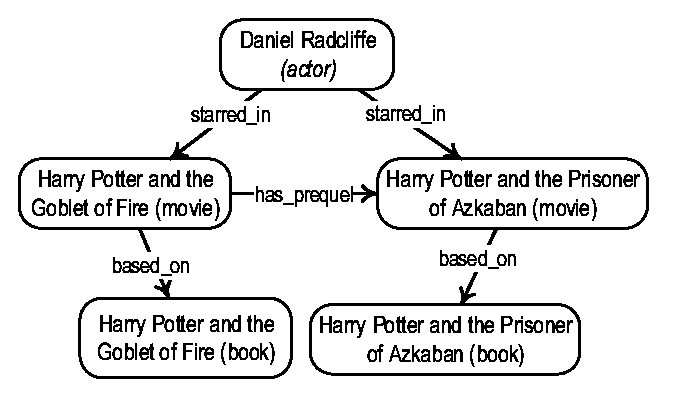
\includegraphics[width=\subfigwidth]{fig/theoretical/example_subgraph_1}\label{fig:context-examples-a}}\\
%         \subfigure[Neighborhood subgraph of size 3 for the entity \textit{Harry Potter}]{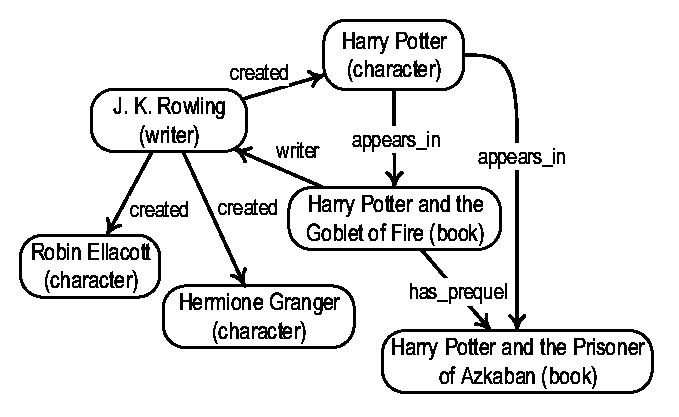
\includegraphics[width=\subfigwidth]{fig/theoretical/example_subgraph_2}\label{fig:context-examples-b}}
%         \caption{Two neighborhood subgraphs for the KG shown in Figure \ref{fig:kg-potter}}
%         \label{fig:context-examples}
%     \end{center}
% \end{figure}

\section{Candidates}\label{sec:theo-candidates}
% As discussed earlier, triples do not make inherent guarantees about the correctness of the knowledge they represent. To represent triples with a higher knowledge quality, this section introduces candidate triples and the notion of fitness in candidate filtering.

\subsection{Candidate triples}
% One can form a syntactically correct triple by just combining two random entities with a random relation. However, chances are that the resulting fact is most likely not correct. Contrary to such a low-quality triple, a candidate triple, or just ``candidate'' for short, is a triple that has been created in such a way that its chance to represent correct knowledge is significantly higher than by mere randomness:

% \defin{Candidate}{
%     Let $\KG = \KGlong$ be a Knowledge Graph, let $s, t \in \Eset$ be two entities and let $r \in \Rset$ be a relation in \KG. We define a candidate as a triple $(s, r, t)$ that has a significantly high chance to represent real-world knowledge, even if it does not exist in \Tset.
% }

% For example, given the KG shown in Figure \ref{fig:kg-potter}, a candidate triple could be \tripleSty{(Daniel Radcliffe, plays, Harry Potter)}. Note that this triple does not exist in the KG in its current state.

\subsection{Fitness function}
% Candidate triples can be generated in a wide manner of ways, that we discuss in more detail in the following chapter. However, it is clear that the number of possible triples, in terms of combinations of entities and relations, is generally orders of magnitude greater than the amount of triples present in any given KG. Therefore, it is possible to generate very large sets of candidate triples that are not yet in a KG.

% As a consequence, it is generally desirable to reduce these sets of candidate triples in a manner that maximizes the preservation of triples with a higher chance to be correct~\cite{shen2022overview, borrego2019}. To formalize this idea, we introduce the concept of fitness function, which assesses the quality of a set of candidate triples in terms of its size and how many correct triples it contains.

% \defin{Fitness function}{
%     Let $\KG =$ $\KGlong$ be a Knowledge Graph, let \Sset{} be a set of candidates and let $\Sset'$ be a set of filtered candidates, with $\Sset' \subseteq \Sset$. We define fitness as a function $fitness(\KG, \Sset, \Sset') \rightarrow \mathbb{R}$ that assigns a score to the filtered set of candidates, with respect to the original set of candidates and KG.
% }

% Since there are many ways to achieve this, we introduce specific instances of fitness functions in the context of KG completion in Chapter~\ref{chap:chai}.

\section{Candidate filtering}\label{sec:theo-rule}
% As previously discussed, it is generally necessary to reduce the size of a set of candidate triples, in order to better assess the remaining candidates for their inclusion in a KG. To achieve this, this section introduces the concept of criterion, and then builds upon it to present the definition of a candidate-filtering rule.

\subsection{Criterion}
% A criterion is an atomic element in candidate filtering. Given a candidate triple in the context of a particular Knowledge Graph, a criterion assigns a binary \texttt{False/True} label to the candidate, denoting whether it should be discarded immediately (\texttt{False}), or tentatively accepted and evaluated more carefully (\texttt{True}):

% \defin{Criterion}{
%     Let $\KG =$ $\KGlong$ be a Knowledge Graph and let the triple $T = (s, r, t)$ be a candidate for $\KG$. We define a criterion as a function $cr(\KG, T) \rightarrow \{False, True\}$ that assigns a binary label to a candidate triple in the context of a KG.
% }

% A given criterion defines a certain method to determine if a candidate triple is likely to be correct or not. For example, a possible criterion would be to accept all candidate triples in which the distance between its two entities is lower than a threshold.

\subsection{Rule}
% In order to express more complex manners of filtering candidate triples, we combine several criteria into a rule. A candidate-filtering rule also produces a binary output for a candidate, in this case, by evaluating multiple criteria and combining their results using conjunctions and disjunctions:

% \defin{Rule}{
%     Let $\KG =$ $\KGlong$ be a Knowledge Graph, let the triple $T = (s, r, t)$ be a candidate for $\KG$, and let $cr_1,\,cr_2,\,\ldots,\,cr_n$ be a number of criteria. We define a rule as a function $rule(\KG, T) \rightarrow \{False, True\}$ resulting of the conjunction and/or disjunction of several criteria, i.e., $cr_1\,(\wedge | \vee)\,cr_2\,(\wedge | \vee)\,\dots (\wedge | \vee)\,cr_n$.

% }

\section{Graph-based features}\label{sec:theo-features}
% To numerically characterize a triple, we propose a set of graph-based features that takes neighborhood subgraphs, reachable entities and paths into account. Due to the possibly large number of different features that can exist, we also introduce the concept of feature groups. Each group can be parameterized to obtain a specific feature, which we call an instance of the feature group.

\subsection{Feature}
% A feature is the simplest way to characterize a triple in the context of the Knowledge Graph it belongs to, by assigning a real number to it according to some operation:

% \defin{Feature}{
%     Let $\KG = \KGlong$ be a Knowledge Graph. We define a feature $f$ as a function $f : \Tset \rightarrow \mathbb{R}$ that assigns a real number to a triple.
% }

% For example, a feature $f$ may convert a triple into the number of entities in the neighborhood subgraph of size 2 of the source entity, i.e., $f : \triple \mapsto |\Eset{}_s^2|$.

\subsection{Feature group}
% Features can have an infinite number of small variations. In our previous example, we mentioned that a feature may leverage the neighborhood subgraph of size 2, but one may conceivably use any subgraph size that is considered appropriate. To be able to express these variations in a more concise way, we define a feature group as follows:

% \defin{Feature group}{
%     Let $\KG = \KGlong$ be a Knowledge Graph. We define a feature group $f_n$ as a function $f_n : \fancy{X} \rightarrow (\Tset \rightarrow \mathbb{R})$ that receives a set of parameters \fancy{X} and returns a feature.
% }

% % TODO: newpage?
% For example, a feature group $f_0$ may return a feature that converts a triple into the number of entities in the neighborhood subgraph of size $n$ of the source entity, i.e., $f_0(n) = f : \triple \mapsto |\Eset{}_s^n|$, where $n$ is a parameter of the feature group. Thus, $f_0(2) : \triple \mapsto |\Eset{}_s^2|$, which is the feature shown in the previous example. Consequently, feature groups allow us to represent a set of very similar features in a more compact way, where the only distinction between said features is a given set of parameters.

\section{Summary}\label{sec:theo-conclusion}
In this chapter, we have described the conceptual framework our proposal relies on. We have defined Knowledge Graphs, triples, paths, distance in a KG and reachability. Furthermore, we have introduced neighborhood subgraphs, candidate triples and fitness functions, as well as candidate-filtering criteria and rules. Finally, we have described graph-based features and their groups.